\chapter{結論}
\section{AIによる楽曲制作の結果}
\subsection{モデルによる生成結果の違い}
\subsection{学習回数による生成結果の違い}
\begin{figure}[h]
    \begin{screen}
    \begin{center}
        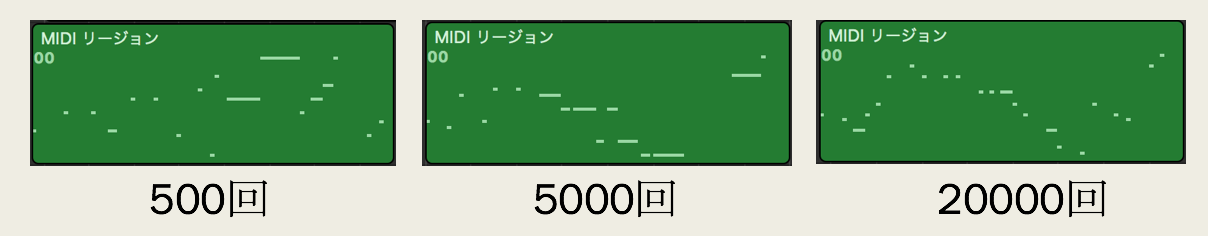
\includegraphics[scale=0.5, clip]{./img/basicMIDI.png}
        \caption{basic\_rnnによる学習回数ごとの生成結果}
        \label{fig:basic_rnnによる学習回数ごとの生成結果}
    \end{center}
    \end{screen}
\end{figure}
\begin{figure}[h]
    \begin{screen}
    \begin{center}
        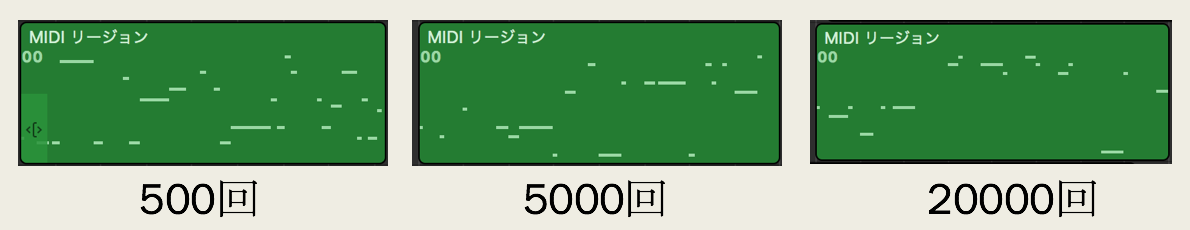
\includegraphics[scale=0.5, clip]{./img/lookbackMIDI.png}
        \caption{lookback\_rnnによる学習回数ごとの生成結果}
        \label{fig:lookback_rnnによる学習回数ごとの生成結果}
    \end{center}
    \end{screen}
\end{figure}
\begin{figure}[h]
    \begin{screen}
    \begin{center}
        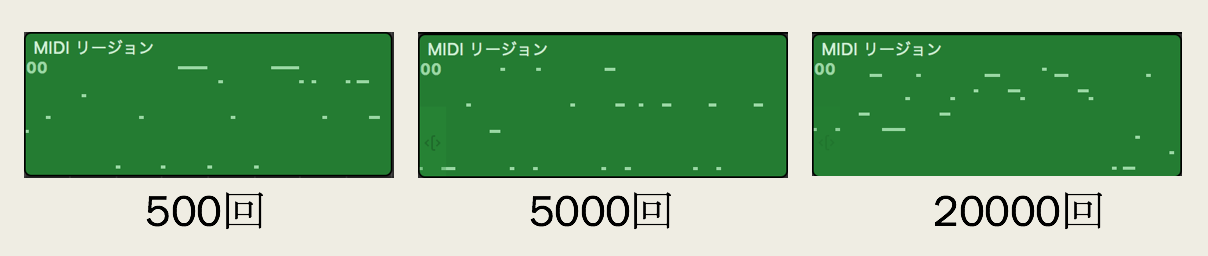
\includegraphics[scale=0.5, clip]{./img/attentionMIDI.png}
        \caption{attention\_rnnによる学習回数ごとの生成結果}
        \label{fig:attention_rnnによる学習回数ごとの生成結果}
    \end{center}
    \end{screen}
\end{figure}
  
\subsection{ノード数による生成結果の違い}
\section{調査結果}

\newpage

\section{今後の課題}
aaa\\